\documentclass{article}

\usepackage{hyperref}
\usepackage[a4paper, margin=1in]{geometry}
\usepackage{cite}
\usepackage{upquote}
\usepackage{parskip}
\usepackage{tikz}
\usepackage{dirtree}
\usepackage{textcomp}

\usepackage{graphicx}

\tikzstyle{plain} = [rectangle, rounded corners, text centered, draw=black]
\tikzstyle{trusted} = [rectangle, rounded corners, text centered, draw=black, fill=red!20]
\tikzstyle{untrusted} = [rectangle, rounded corners, text centered, draw=black, fill=yellow!20]
\tikzstyle{arrow} = [thick,->,>=stealth]

\title{Kerberos-based single sign-on with delegation for web applications}
\author{Daniel Carter}
\date {\today}

\begin{document}
\maketitle

\section{Introduction}

\subsection{Web application security}
Many web applications are built around a database, which is used by the application framework to store user data and load it for display to the user. In general, the user logs in using a username and password (which is checked by the web app framework itself), and the application then makes database queries on the user's behalf, processes the results, and displays them to the user in a suitable way.

In this scenario, the application framework has the ability to read and write arbitrary data in the database, and the only thing which prevents a malicious user from accessing data which they are not authorised to read is the application code itself. This is potentially problematic, since web app authors are often not security experts and may accidentally cause data to be visible to the wrong users. Some examples of how this can occur include:

\subsubsection{SQL injection}
This is a form of command injection attack (which are currently number 1 in the OWASP \textit{Top 10 Web Application Security Risks} list\cite{OWASP10}). This occurs when an application uses a template database query such as
\begin{verbatim}
SELECT * FROM records WHERE username='$user';
\end{verbatim}
and replaces \verb+$user+ with a string that the user provides. However, with insufficient checking of parameters, a user can supply a string such as
\begin{verbatim}
' OR 1=1; --
\end{verbatim}
resulting in a total query of
\begin{verbatim}
SELECT * FROM records WHERE username='' OR 1=1; --';
\end{verbatim}
which returns the records of all users (since \verb+1=1+ is always true).

The following diagram represents an example of a typical current setup, and the problems that can be caused if an SQL injection vulnerability is present:

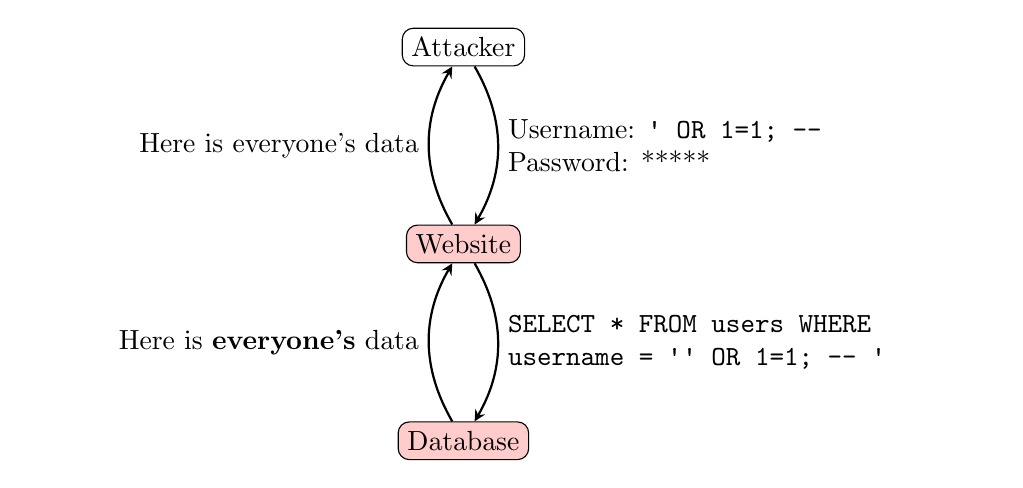
\begin{tikzpicture}[node distance=2.5cm]
  \node (user) [plain] {Attacker};
  \node (webserver) [trusted, below of=user] {Website};
  \node (database) [trusted, below of=webserver] {Database};

  \draw [arrow, bend left] (user) edge node[right] {\parbox{0.5\textwidth}{Username: \texttt{\textquotesingle \ OR 1=1; --} \\ Password: *****}} (webserver);

  \draw [arrow, bend left] (webserver) edge node[right] {\parbox{0.5\textwidth}{\raggedright \texttt{SELECT * FROM users WHERE \\ username = \textquotesingle\textquotesingle \ OR 1=1; -- \textquotesingle}}} (database);

  \draw [arrow, bend left] (database) edge node[left] {\parbox{0.4\textwidth}{\hfill Here is \textbf{everyone's} data}} (webserver);
  \draw [arrow, bend left] (webserver) edge node[left] {\parbox{0.4\textwidth}{\hfill Here is everyone's data}} (user);        
\end{tikzpicture}

\subsubsection{Master password leakage}
There are many variations on this depending on exactly what was leaked, but these usually enable any malicious user to arbitrarily read and write from the database. Since the web app itself has these capabilities, it usually has a single username and password which it uses to authenticate with the database, and these are usually stored in a simple configuration file. If the webserver is misconfigured such that the configuration file is visible over the internet, or if the file is accidentally checked into a public source control repository, an attacker can read this file, connect to the database server and read out all the data.

To demonstrate how significant a problem this is, a number of companies (such as GitGuardian\cite{GitGuardian}) have been set up simply to monitor online repositories for leaked security keys, and warn their owners. As a case in point, when setting up the test site for this project, the Django \texttt{settings.py} file initially contained a secret key that would allow an attacker to forge cryptographic signatures and so break the security of the application to an extent (but \textbf{not} gain full access to the database due to the application's structure, as detailed below). Although the key was moved to a file outside the repository (and changed, so that knowledge of the old secret key would be of no use to an attacker) before any files were made public, the mere existence of the secret key in a prior commit caused a warning email to be sent to me by GitGuardian within 70 minutes of changing the repository's visibility:

\includegraphics[width=9cm]{01-gitguardian.png}

Even though this service only offers after-the-fact detection (a service which has genuinely leaked a secret key must quickly change this key everywhere it is used, and the site may still have been compromised in the meantime), the fact that businesses exist to perform these scans, and seemingly scan all public GitHub repositories to alert their owners, indicates the severity of this issue.

\subsubsection{Legal Implications}
As well as being commercially and reputationally damaging, unauthorised access to data can result in severe legal penalties: the Data Protection Act 2018 specifies a fine of up to 2\% of a company's global turnover (or 10 million Euros, if that is greater) may apply in cases of unauthorised disclosure of personal data\cite{GDPR}. Developing technologies that mean the web app does not have to be trusted with all data can significantly reduce the risk of these types of disclosure.

\subsection{Website Sign-on Systems}
A further disadvantage of having a ``local'' system of checking passwords on each website is that users are then expected to memorise a large number of different passwords, since otherwise a compromise of the password database of one website would allow the attacker to impersonate users on any other website where they had used the same password. Especially where several websites are ``connected'' in some way (e.g.\ by all being associated with the same organisation), a \textit{single sign-on} system can offer significant benefits.

A single sign-on (SSO) system generally consists of an authentication server, which collects a password (or some other security token) from the user and verifies the user's identity. When a user wishes to log on to a site which uses that SSO system, the user is redirected to the authentication server to log in. Assuming the login is successful, the user is redirected back to the site, along with some kind of unforgeable token to indicate that the authentication server has verified the user's identity.

Note that these steps only provide \textbf{authentication} of the user (i.e.\ that the person logging into the site is actually user $X$). \textbf{Authorisation} (i.e.\ checking whether user $X$ is entitled to access the site) must be done separately by the sites themselves.

The University's Raven authentication service is an example of an SSO system; numerous similar systems exist (including OAuth2, which also has the ability to do a form of ``delegation'' to allow one server to request resources from another, on behalf of the user\cite{Oracle-OAuth2}).

\subsection{Project Summary}
This project aims to produce an authentication system for web applications, such that a user can authenticate to a web application using a Kerberos ticket and the web application can use this ticket to obtain the user's data from a database.

Apart from having a Kerberos ticket in the first place, this is set up to be completely transparent to the user -- all they need to do is to visit the website and the authentication process will be carried out automatically (with the minor caveat that Kerberos authentication must be specifically enabled in most web browsers, although in a corporate environment this could be done centrally).

As a demonstration of this in practice, the project includes an example file-browser application that performs all authentication and authorisation via Kerberos tickets and database permissions, rather than implementing the security in the web app.

\subsection{Related Work}
The core Kerberos system and its extensions are described in a series of RFCs, several of which are relevant to this project:

\begin{itemize}
\item
  RFC 2478\cite{RFC2478} describes the \textit{Simple and Protected GSS-API Negotiation Mechanism} (SPNEGO) which gives a (relatively generic) overview of negotiation-based authentication, where a server can provide information on what authentication methods it supports and the client can complete the authentication process using one of these methods. This RFC illustrates examples of how the authentication process works, but is not tied to a particular protocol, and so is an important description of many of the overall concepts referred to in this project.
\item
  RFC 2743\cite{RFC2743} (along with several earlier RFCs) defines the current version of the Generic Security Service API (GSS-API) conceptually, using an exchange of tokens to prove identity and incorporating the concept of security tokens being delegatable to another system or process. Principles stated here include that of the tokens being ``opaque from the viewpoint of GSS-API callers'', where the user of a system simply requests a ticket and then passes it to the appropriate service without the user attempting to extract the contents of the ticket. RFC 2744\cite{RFC2744} lays out a concrete API for RFC 2743 in the form of C language bindings.
\item
  RFC 4178\cite{RFC4178} describes, at a conceptual level, a negotiation framework for GSS-API systems to select an authentication system which they are both compatible with. Under this setup, the system initiating a connection offers a set of mechanisms which it can use to connect, with an order of preference. The system being connected to can then use the highest-preference system which it is capable of using, or refuse the connection if none of the suggested mechanisms are suitable.
\item
  A later RFC (RFC 4559\cite{RFC4559}) refers to a Windows-based system which allowed a user to log into a web application, from which a suitably equipped application could delegate the ticket to another system such as a database server. This was included by Microsoft in IIS 5.0 by virtue of adding a ``Negotiate'' extension to the HTTP protocol for use with Kerberos, and permitted a user to log in to the website without needing a password as described above in the aims for this project.
\end{itemize}

The ``HTTP Negotiate'' extension was subsequently included in various open-source web browsers. It also has some support in the Apache web server, and the aim of this project is effectively to replicate Microsoft's setup using an open-source web framework (Django) in conjunction with the Apache web server and any client web browser which supports the Negotiate extension.

\section{Preparation}

\subsection{Kerberos}
The Kerberos protocol works based on a system of \textit{tickets}, which are managed by a \textit{Key Distribution Centre} (KDC). The basic requirement of the system is to allow a centralised database of users (for example, the main login directory in an office) who can demonstrate their identity in order to log in to applications and services, but \textit{without} having to store or transmit passwords or other long-term secrets on potentially untrusted machines.

The basic workings of the protocol are as follows:

\begin{itemize}
\item
  A user initiates a session by reqesting a Kerberos ticket from the KDC, authenticating using their password.
\item
  The KDC returns a \textit{ticket-granting ticket} (TGT), and returns it encrypted using the user's password.
\item
  The user decrypts the TGT, and the user's machine can then discard the stored password.
\item
  When the user wants to access a service, they send the TGT back to the KDC along with an identifier for the service which they want to use.
\item
  The TGT grants the user a \textit{service ticket}, which the user then passes on to the service. The service is then able to use that ticket for authentication.
\end{itemize}

The following listing shows a client which has obtained both a TGT and a service ticket. The ticket in the first line (\verb+krbtgt/LOCAL@LOCAL+) is the \textit{ticket-granting ticket} which the client obtained when first authenticating to the KDC, and the second (\verb+HTTP/krbsite.local@LOCAL+) is a \textit{service ticket} to log in to the \verb+HTTP+ service on \verb+krbsite.local+ (i.e.\ to access the web page hosted on that server).

\begin{quote}
\begin{verbatim}
daniel@Daniel-Laptop:~$ klist
Ticket cache: FILE:/tmp/krb5cc_1000
Default principal: dcc@LOCAL

Valid starting     Expires            Service principal
02/04/21 15:36:01  03/04/21 01:36:01  krbtgt/LOCAL@LOCAL
	renew until 03/04/21 15:36:01
02/04/21 15:36:07  03/04/21 01:36:01  HTTP/krbsite.local@LOCAL
	renew until 03/04/21 15:36:01
\end{verbatim}
\end{quote}

\subsection{Kerberos Ticket Delegation}
In addition to use for authentication, Kerberos supports a method of \textit{delegating} tickets. This means that a principal $A$ can pass a ticket to a service $X$ as a means of authentication, and $X$ can pass the ticket on to a third system $Y$ to request resources on the user's behalf.

This is valuable because it means that $X$ can access resources which ``belong'' to $A$, without $X$ needing to have direct access to $Y$. This means that less trust in $X$ is needed (since it does not need privileged access to $Y$), and so the types of attacks discussed above become much less likely.

\subsection{Project Structure}
This project demonstrates a web application that uses Kerberos authentication and delegation to fetch data from a database and display it to the user, in the form of a basic file browser-type application. It also includes a component which performs the necessary setup tasks (setting up SQL permissions), so that all that is required for the user of the application is to:
\begin{itemize}
\item
  Set up a Django app with the appropriate models (in the example web app, the models are files and directories, plus associated tables to hold permissions)
\item
  Run the normal Django \texttt{migrate} command to set up the database
\item
  Use the web interface (created as part of this project) to set up appropriate access controls
\end{itemize}

The overall structure of the authentication process is as shown below, noting that the application itself does not have any other access means of accessing the database, so an attack such as the one depicted above cannot take place.

Since the same KDC can be used for many websites where the users all have a login to the same Kerberos realm, the system also functions as a single sign-on system (using the Kerberos ticket as proof of identity). As detailed in sections 2 and 3, this does \textbf{not} mean that any of the individual websites need to be given access to the user's password, or that they are able to arbitrarily impersonate the user on other systems. The possibility of delegating tickets in a controlled manner means that the website shown can fetch data from the database on behalf of the user, but not from other systems which it has not been authorised to access.

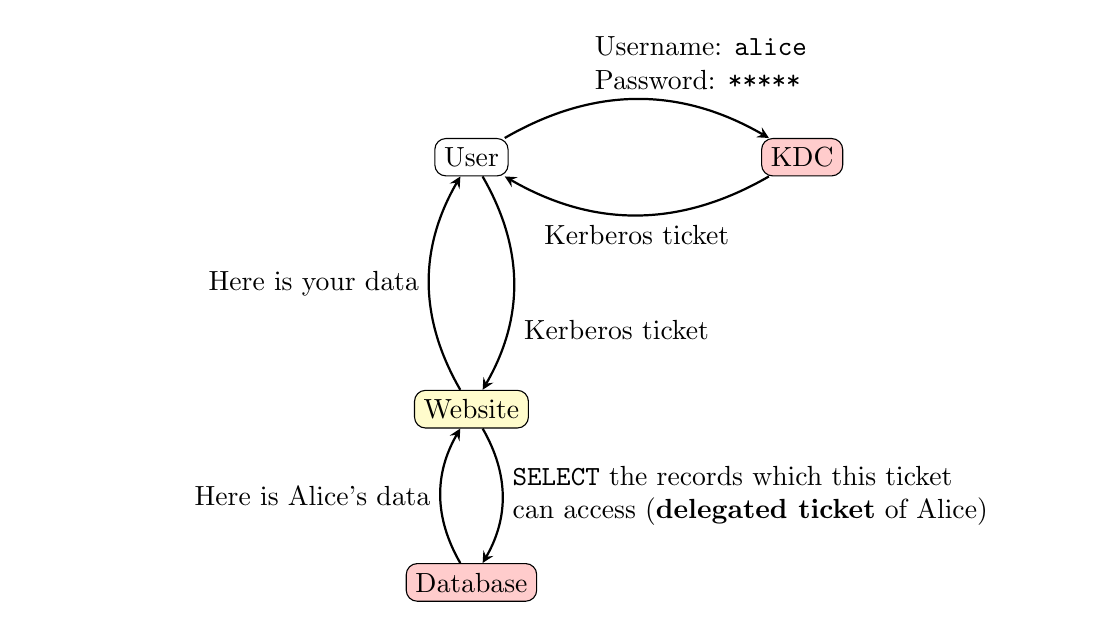
\begin{tikzpicture}[node distance=2.2cm]
  \node (user) [plain] {User};
  \node (webserver) [untrusted, below of=user, yshift=-1cm] {Website};
  \node (database) [trusted, below of=webserver] {Database};
  \node (kdc) [trusted, right of=user, xshift=2cm] {KDC};

  \draw [arrow, bend left] (user) edge node[above, xshift=2.5cm] {\parbox{0.5\textwidth}{Username: \texttt{alice} \\ Password: \texttt{*****}}} (kdc);

  \draw [arrow, bend left] (kdc) edge node[above, yshift=-0.5cm] {Kerberos ticket} (user);

  \draw [arrow, bend left] (user) edge node[right, yshift=-0.6cm] {Kerberos ticket} (webserver);

  \draw [arrow, bend left] (webserver) edge node[right] {\parbox{0.5\textwidth}{\raggedright \texttt{SELECT} the records which this ticket can access (\textbf{delegated ticket} of Alice)}} (database);

  \draw [arrow, bend left] (database) edge node[left] {\parbox{0.4\textwidth}{\hfill Here is Alice's data}} (webserver);
  \draw [arrow, bend left] (webserver) edge node[left] {\parbox{0.4\textwidth}{\hfill Here is your data}} (user);
\end{tikzpicture}


\section{Implementation}

\subsection{System Structure and Repository Overview}
The core of this project is a Django web app, which is able to both perform the necessary setup steps to get the system working and (as a separate component) demonstrate the working of the system.

The structure of the directories involved is as shown below. The basic directory layout is as produced by the Django project setup procedure, with some files having ``stubs'' automatically generated by this process.

\dirtree{%
.1 /.
.2 files.
.3 admin.py.
.3 apps.py.
.3 \_\_init\_\_.py.
.3 migrations.
.4 \_\_init\_\_.py.
.3 models.py.
.3 templates.
.4 files.
.5 index.html.
.5 listing.html.
.3 tests.py.
.3 urls.py.
.3 views.py.
.2 krbsite.
.3 asgi.py.
.3 filedb\_router.py.
.3 \_\_init\_\_.py.
.3 middleware.py.
.3 settings.py.
.3 urls.py.
.3 wsgi.py.
.2 managedb.
.3 admin.py.
.3 apps.py.
.3 forms.py.
.3 \_\_init\_\_.py.
.3 models.py.
.3 templates.
.4 managedb.
.5 index.html.
.5 result.html.
.5 table\_mapping.html.
.3 tests.py.
.3 urls.py.
.3 views.py.
.2 manage.py.
}

In keeping with the principle that the web app should simply be a ``view'' onto the main database (and also the limited privileges that the app itself has for writing to the database), Django uses a separate database for recording session information and associated ``housekeeping'' data, but not any of the actual records which have access control applied to them.

For ease of setup (since this is not a significant aspect of the project), this was done using a simple SQLite database, although the setup did require a Django \texttt{AuthRouter} to make sure that queries are always directed to the appropriate database: see \hyperref[sec:appendix1]{Appendix 1} for more details and code.

\subsection{SPNEGO}
SPNEGO (Simple and Protected GSSAPI Negotiation Mechanism) is a mechanism which uses a single packet exchange to itentify a suitable protocol to authenticate the user with. In practice, it is usually used with either NTLM (a challenge-response protocol, whose cryptography can be easily broken using current technology and so which is vulnerable to attack) or Kerberos, and the server can specify which protocols it is willing to accept.

For example, using the \verb+mod_auth_gssapi+ Apache module used here, the following directive ensures that only Kerberos (\texttt{krb5}) authentication will be accepted for GSSAPI:

\begin{verbatim}
GssapiAllowedMech krb5
\end{verbatim}

Note: a full copy of the \verb+.htaccess+ file which configures many options in Apache for this project, is included in \hyperref[sec:appendix2]{Appendix 2}.

\subsection{Kerberos Backend}
The KDC and related Kerberos backend services are a significant component of the system, and form part of the \textit{trusted computing base} of the setup (i.e.\ the parts of the system which, if compromised, could allow the security of the whole system to be compromised). Although not actually requiring any new software development (since in a real situation this backend would already exist, for instance as an Active Directory server), arranging a suitable test setup with the right permissions was required for the project.

\subsubsection{Basic MIT Kerberos Backend}


\subsubsection{Connecting to an LDAP Server}

\subsection{Kerberos Ticket Delegation}
Another major aspect of this project is how a ticket can be \textit{delegated} from one server to another, such that the ticket used to log into the web app can be used to authenticate to another system.

\subsubsection{Unconstrained Delegation}
The traditional, and simplest, method for delegation is simply for the user $A$ to pass their ticket-granting ticket to the service $X$. $X$ can now behave as though it were $A$, and access any resources to which $A$ has access by simply presenting $A$'s ticket-granting ticket to the KDC and requesting a suitable service ticket.

In MIT Kerberos, this is achieved by marking service $X$ with the \verb+ok-as-delegate+ flag, which ``hints the client that credentials can and should be delegated when authenticating to the service''\cite{KDC-conf-docs}.

Despite seemingly being no better than $A$ simply giving a password to $X$ (so that $X$ can log in ``as'' $A$ when accessing $Y$), this scheme offers some advantages:

\begin{itemize}
\item
  Kerberos tickets are time-limited, so if $A$ no longer wishes to allow $X$ to access resources, all $A$ has to do is wait for any delegated tickets which $X$ currently holds to expire (and not send any more). This contrasts with passwords which are valid indefinitely and may well not be straightforward to change in a complex corporate network.
\item
  Some limitations are placed on what can be done with the tickets. Although $X$ can use the TGT to get a service ticket to any other system $Y$ that $A$ can access, $Y$ does not automatically have the right to delegate this ticket further. If $Y$ does \textbf{not} have the \verb+ok-as-delegate+ flag set, then $X$ can \textit{access} $Y$ on $A$'s behalf but not allow $Y$ to perform actions for $A$ on some other server $Z$. If $Y$ is not well-trusted, this can be a significant benefit.
\end{itemize}

While the second of these advantages is significant, it may still not offer enough access control over the network. In particular, $A$ cannot give $X$ the ability to delegate to $Y$ without also giving $X$ the ability to delegate to \textbf{any} other service which $A$ has access to. In many cases this would be too great a risk; it may well be desirable to allow $X$ to fetch $A$'s work documents from $Y$ to display them in a web app, but not to allow $X$ to retreive $A$'s financial records from another system $Z$ within the same Kerberos realm.

In this case, constrained delegation offers a far more controllable method of only allowing services to delegate tickets in particular ways, at the expense of a more complex setup for managing applications.

\subsubsection{Constrained Delegation (S4U2proxy)}
The \textit{Service for User to Proxy} (S4U2proxy) system is an extension to the basic Kerberos setup that allows one service $X$ to obtain a ticket to another service $Y$ (on behalf of a principal $A$) in a controlled manner. Once service $X$ has been marked as ``permitted'' to obtain tickets for service $Y$, it can do so simply by making a request to the KDC, without having any need to know the user's Kerberos password\cite{MS-s4u2}.

Unlike with unconstrained delegation, here the ticket-granting ticket is not passed over to $X$; instead, $X$ is given a service ticket from $A$ as normal (to prove $A$'s identity and that $A$ wishes to connect to $X$). When $X$ needs to access $Y$ on behalf of $A$, $X$ \textit{submits the service ticket} to the KDC. If the permissions in the KDC are set appropriately, it is able to give $X$ a ticket to $Y$ on behalf of $A$.

This requires a more complex setup of permission models in the KDC than simply a list of principals, since the KDC must now decide which services can delegate tickets to which others. The default back-end for MIT Kerberos does not support this, but moving the user data into an LDAP server and using this as the data source allows the relevant \texttt{krbAllowedToDelegateTo} permission to be set on the user\cite{KRB-DELEG}.

In addition to the advantages described above for unconstrained delegation, there are some further advantages here:

\begin{itemize}
\item
  Access control can be almost completely customized. The system can now be set up so that $A$ can log into $X$ and have a Kerberos ticket delegated to $Y$, or log into $P$ and have a ticket delegated to $Q$, but not allow $X$ to delegate to $Q$. There is no simple set of ``privileged'' applications which are allowed to perform (all) delegation, but a customizable set of permissions between systems.
\item
  The number of powerful ticket-granting tickets that are stored in systems on the network is reduced. If an attacker gains access to $X$, the attacker will, at most, get service tickets for all users who have recently logged into $X$ (i.e.\ who have logged in and whose stored tickets have not yet expired), and delegated service tickets to the services which $X$ is allowed to. The attacker does not get a ticket-granting ticket to use on arbitrary applications.
\end{itemize}

In this project, the permitted delegation patterns are described using records in the LDAP database. The following pattern is therefore used to allow the web server on \verb+krbsite.local+ to delegate to PostgreSQL on \verb+krb.local+ (i.e.\ set the \texttt{krbAllowedToDelegateTo} attribte on \verb+HTTP/krbsite.local+ to \verb+postgres/krb.local+):

\begin{verbatim}
dn: krbPrincipalName=HTTP/krbsite.local@LOCAL,cn=LOCAL
,cn=krbContainer,dc=local
changetype: modify
add: krbAllowedToDelegateTo
krbAllowedToDelegateTo: postgres/krb.local@LOCAL
\end{verbatim}

\subsubsection{S4U2self}
This description is included here for completeness (because of its similar name) although it is \textbf{not} a true method of delegating tickets.

The Microsoft standard document for S4U2self\cite{MS-s4u2} states that:

\begin{quote}
  The S4U2self extension allows a service to obtain a service ticket to itself on behalf of a user. The user is identified to the KDC using the user's name and realm. Alternatively, the user might be identified based on the user's certificate.
\end{quote}

In effect, Kerberos authentication is bypassed completely and the server $X$ is able to get a ticket for $A$ simply by specifying $A$'s user name. This may be useful in some situations if not all clients can use Kerberos, but it offers a significantly weaker security model (since $X$ can now obtain service tickets for any user) and so if $X$ is compromised then records from all users can be gathered. As the aim of this project is to reduce the amount of trust placed in applications such as $X$, S4U2self is not relevant to this goal and will not be considered further.

The ability of $X$ to get a delegatable ticket using S4U2self can be controlled in the KDC, and so (for example) the following command is used to stop the web server from being able to to so:

\begin{verbatim}
modprinc -ok_to_auth_as_delegate HTTP/krbsite.local@LOCAL
\end{verbatim}

\subsection{Credential Cacheing in the Web Server}
When user $A$ provides a Kerberos ticket for to service $X$ as part of the negotiation process, the ticket can either be discarded immediately following the completion of the request (including after any necessary delegation has occurred) or be cached by the server for future use.

The first of these offers a ``purer'' Kerberos setup, since the web server does not need to store any state and can simply use a ticket provided by the user on each request. However, this approach significantly limits the performance of the system:
\begin{itemize}
\item
  Since the basic HTTP Negotiate setup requires a multi-stage ``handshake'' before communication can begin, each request to the web server now becomes at least two requests. This potentially doubles the access time to the website, as well as consuming extra network bandwidth and placing additional load on the web server. Given that individual web pages often consist of a number of elements (e.g.\ each image on the page would require a new request and another round of HTTP negotiation) this is certainly non-ideal.
\item
  Kerberos ticket files are potentially large (especially those issued by Windows-based systems\footnote{As a (somehwat simplistic) illustration of this, obtaining a Kerberos ticket from my test application (running MIT Kerberos) produced a credential cache of size 650 bytes. Obtaining a ticket from the University's Active Directory server \texttt{BLUE.CAM.AC.UK} resulted in a file size of 1536 bytes, or over double the size of the MIT Kerberos ticket.}) and having to include the full ticket in each request may take up significant additional bandwidth. This may cause problems if users are on slow or quota-controlled network connections, and further increases the demand on the server.
\end{itemize}

See the evaluation for more discussion of the problems caused by using this approach.

One possible solution would be for the web server to place the ticket itself into a cookie that is sent to the client. This would mean that each request could take place as normal (with the client providing the cookie and the server extracting the ticket from the cookie to use for authentication) and so solve the first of the issues above, but still result in (potentially) large cookie files being sent around and adding a lot of overhead to every request.

The solution generally adopted here is to cache the tickets on server $X$ and send a (short) session cookie to $A$ so that $X$ can identify $A$ when $A$ connects again and provides the same cookie. However, since this cookie does not carry any information beyond acting as an identifier, $X$ must store a copy of $A$'s Kerberos ticket to use when $A$ connects to the server on subsequent occasions.

Ignoring two Windows-specific mechanisms, MIT Kerberos offers five methods of storing credential caches\cite{MIT-ccache-types}:

\begin{itemize}
\item
  \textbf{DIR} (directory) mode places all tickets in the supplied credential cache into a particular directory. In this case (since $A$ only needs to supply one ticket to $X$) this has no advantage over \textbf{FILE}.
\item
  \textbf{FILE} mode stores the credential cache into a file on the server's filesystem. This offers the best built-in support in existing modules, but its default configuration is vulnerable to having tickets stolen if the webserver is compromised (see below).
\item
  \textbf{KCM} mode was recently added to MIT Kerberos, and uses a specific daemon process to manage credential caches. Although potentially offering advantages over simpler systems (and being less OS-specific than \textbf{KEYRING}), it is still primarily tied to the UID of a user account and so does not offer much security between different tickets held by the same server user. Since having a separate login account on the web server for each database user would normally be impractical, this limits the usefulness of this option.
\item
  \textbf{KEYRING} mode uses a feature of the Linux kernel to store credentials in an area of private memory. This has the advantage over many of the methods listed here that a kernel keyring can be made process- or thread-specific and so prevent other threads gaining access to private credential caches.

  However, the process model used by the Apache web server introduces some difficulties in this situation. Since the same Apache worker process may be used to process different (unrelated) requests at different times, it is important that these requests do not have access to the credential caches saved for the previous requests using that thread. Since the thread and process IDs will remain the same for future requests, this is difficult to acheive.

  Further, the \verb+mod_auth_gssapi+ module is currently only designed to work with file-based caches (the \verb+mag_store_deleg_creds+ function prepends \texttt{FILE:} to any input it is given, and the \verb+gss_store_cred_into+ function which is then called is only set up to write output data into a file). It would be possible to modify this to work with kernel keyrings (and this was something I investigated as part of the project), but eventually a file-based approach (with some additional protections to keep tickets private, as detailed below) was used.
\item
  \textbf{MEMORY} caches, which are conceptually similar to keyring-based caches except they are not Linux-specific and offer less granularity in setting access permissions. Many of the same issues described above also apply to this cache type, particularly in relation to removing access from threads.
\end{itemize}

Although the best-supported by current systems, file caches are non-ideal (in their default configuration) because they are normally placed in a directory whose contents can be enumerated and read by any other process running as the same user. In this case, this means that a web app which was compromised to allow code execution in the context of a user's web app session could access tickets belonging to other users who had logged in recently and whose tickets were still cached.

In order to improve this, I added an option to \verb+mod_auth_gssapi+ (\texttt{GssapiDelegCcacheRandom}) which adds a random 16-character string to the credential cache name. When combined with \texttt{0300} directory permissions (i.e.\ \texttt{d-wx------} -- the owning user can write to the directory and traverse it to find files if the filename is known, but not read the list of files in it), this means that tickets can only be accessed by knowing the credential cache filename, which is passed to the web app and on to the Kerberos library via an environment variable. Therefore, one instance user's of the web app is not able to obtain tickets belonging to another.


\subsection{SQL Access Control}
A core aspect of this project is the ability to shift access control from the web app itself to the SQL server. Most SQL server applications contain permissions models which allow selective access to data, and there are often a number of ways of achieveing this (especially since they are not very well standardised across SQL implementations). As this project specifically uses PostgreSQL, I evaluated a number of supported methods to determine how best to implement the security protocol.

\subsubsection{\texttt{SECURITY DEFINER} functions}
A PostgreSQL function with \texttt{SECURITY DEFINER} in the signature runs ``as'' the user creating the function, regardless of who executes it\cite{postgres-SEC_DEF} (in a similar way to how the \texttt{setuid} bit works in Unix). This allows the database owner to create a function which can read the whole table and when run, perform some check based on the user calling it and return appropriate results.

This approach requires some caution since the \texttt{SECURITY DEFINER} property also redefines the \verb+current_user+ variable (which normally contains the username of the user executing a query) to the user who defined the function, although this can be worked around using \verb+session_user+ instead. Once this is taken into account, such a procedure can be used to return files where the current user has an appropriate entry in a permission table.

While very flexible, this approach is is not easily integratable into frameworks such as Django, which are designed to execute queries on tables rather than (effectively) making function calls to an API. Since the goal is to allow the user to set up a Django web app which works using existing models, this setup is non-ideal.

\subsubsection{SQL views}
These effectively allow a new table to be created out of a view over an existing table. Using syntax such as the following, it is therefore possible to construct a new table which only has the calling user's files visible; the user can then be granted access to this view (which automatically selects files based on their own username) and does not then need to have any access to the original table. For web application purposes, it can be queried just like any other table.

\begin{verbatim}
CREATE VIEW my_files AS
SELECT f.*
FROM files_file f, files_permission p
WHERE f.id = p.file_id
AND p.owner = user;
\end{verbatim}

While less significant than for \texttt{SECURITY DEFINER} functions, views also introduce difficulties for interfacing with Django since each database table now needs to have two entries in the Django model setup (one for the table itself and one for the view). Using abstract classes and inheritance allows some reduction in the amount of duplication, but this is still non-ideal.

\subsubsection{Use of \texttt{ON SELECT} to redefine selection}
PostgreSQL also allows rules to be created which effectively redefine actions on tables. For example, a rule could be used to replace the default \texttt{SELECT} rule on the table storing file information with one that checked user permissions.

However, this is likely to introduce unnecessary complexity (particularly with ensuring that administrators can still access data as necessary, for example). For these reasons, the PostgreSQL documentation considers it ``better style to write a \texttt{CREATE VIEW} command than to create a real table and define an \texttt{ON SELECT} rule for it''\cite{postgres-CREATE_RULE}.

\subsubsection{Row-level security}
The final method considered, and the one which turned out to be best-suited to this problem, was PostgreSQL's row-level security constructions. These allow policies (defined by the database owner) to determine who can view which rows in the database.

There are two forms of policy, which are applied in different cicumstances\cite{postgres-policy}:
\begin{itemize}
\item
  \texttt{USING} policies, which work on existing rows to determine whether users are allowed to view and/or update the contents of a row. This is used for the main data tables (since the main concern is the confidentiality of file data), where the following lines of code allow users to view and update files which they have permission records for:

\begin{verbatim}
# Enable row-level security on the relevant table
cursor.execute("""ALTER TABLE %s ENABLE ROW LEVEL SECURITY"""
        % (source_table))
# Only allow users to view and edit files which they have permission to see
cursor.execute("""CREATE POLICY %s_view ON %s
USING (%s IN (SELECT %s FROM %s WHERE %s = session_user))"""
        % (source_table, source_table, source_column, perm_column, perm_table,
           owner_column))
\end{verbatim}

  With a \texttt{USING} policy, a row which fails the policy is not visible to the user and so cannot be accessed.

\item
  \texttt{WITH CHECK} policies, which are designed to protect insertion of new rows. These are more suited to protecting the integrity of data (by stopping unauthorised additions) and so are used in this application for the permission tables. Since an attacker could otherwise insert permissions to allow them to read arbitrary files, this is another critical part of the security model:

\begin{verbatim}
# Also enable row-level security on the permissions table
cursor.execute("""ALTER TABLE %s ENABLE ROW LEVEL SECURITY"""
        % (perm_table))
# Only allow users to set permissions where they already have access to that file
cursor.execute("""CREATE POLICY %s_view ON %s FOR INSERT
WITH CHECK (%s IN (SELECT %s FROM %s WHERE %s = session_user))"""
        % (perm_table, perm_table, perm_column, perm_column, perm_table,
           owner_column))
\end{verbatim}

  A further special-case policy allows newly created files (with no current owner) to have permissions assigned. With this type of policy, an error is generated if a user tries to create entries without the authority to do so.

\end{itemize}

Note that the table names above are separately verified by the application before being placed into these database queries to avoid SQL injection being directly possible here, but also that logging in as the database administrator to perform these types of actions inherently involves having full access to the database and so it is impossible to remove all SQL injection risks if the application is compromised \textbf{while} the set-up phase is going on.

The row-level security model runs in parallel with the standard SQL permissions model and both systems must allow access for an action to be allowed. Thus, to only allow read-only access to selected rows, a \texttt{USING} policy can be set up to determine row accesses, and the user concerned only granted \texttt{SELECT} (and not \texttt{UPDATE}) access to the table. This is employed in the application to restrict malicious modifications to permission entries.

These policies (which work by executing a piece of SQL code on attempted access to determine whether access and/or modification of a piece of data by the current user is allowed) are effectively similar to Trusted Procedures in a Clark-Wilson security model, where data can only be modified by particular procedures which enforce constraints on the data. This therefore allows something of a separation of authentication (logging into the database, via Kerberos) and authorisation (where the permission table describes what access is permitted).

\subsection{The database setup application}
As the most significant component of software produced for this project, the database setup application is designed to allow a website administrator to easily set up SQL permissions such that other Django applications (including the file browser example app) work with minimal changes.

This application first needs to gather information from the user to allow a ``matching'' of data and permission tables (i.e.\ to determine which table holds permission records for a given table of data). This is clearly dependent on where there are appropriate table relationships already set up (a permission table must contain a foreign key to the data table), and PostgreSQL exposes this information via an internal \verb+information_schema+ table.

Therefore, executing the following query on a given model (using the \verb+model_data+ paramaters which are incorporated into the query) provides a set of candidate permission tables where such a foreign key exists:

\begin{verbatim}
cursor.execute("""SELECT dst.table_name, dst.column_name
    FROM information_schema.constraint_column_usage src,
         information_schema.key_column_usage dst,
         information_schema.table_constraints constraints
    WHERE src.constraint_name = constraints.constraint_name
    AND constraints.constraint_name = dst.constraint_name
    AND constraints.constraint_type = 'FOREIGN KEY'
    AND src.table_name = %s
    AND src.column_name = %s""",
    [model_data['table'], model_data['primary_key']])
\end{verbatim}

The application then performs a further query to the \verb+information_schema+ table to identify columns in these candidate tables which could be used to store the user's identity in a permission element. Because Django itself has no knowledge of the database's users, these are simply stored as string values (\texttt{character} or \texttt{character varying} in PostgreSQL nomenclature) in the database:

\begin{verbatim}
cursor.execute("""SELECT column_name
    FROM information_schema.columns
    WHERE table_name = %s
    AND data_type LIKE 'character%%'""",
    [table])
\end{verbatim}

\subsection{Kerberos access to PostgreSQL}
Although PostgreSQL includes Kerberos-based authentication via the GSSAPI framework\cite{postgres-GSSAPI}, the client which connects it to Django (and to most other applications) currently does not offer a choice of which ticket to use and simply takes a stored ticket from the system's default \texttt{ccache} location. This is obviously unsatisfactory in the case of an application where many user's tickets will be stored and the application must use the appropriate ticket each time, and so I have added a patch to the PostgreSQL client library to perform this.

Django's interactions with PostgreSQL are achieved using the \texttt{psycopg} library, which forms the basis for the PostgreSQL backend which comes with Django. However, much of the actual library functionality is simply a wrapper around the C-based \texttt{libpq} library, which is provided as part of PostgreSQL and manages the actual interaction with the database server.

% TODO: Some more thorough coverage of the Python implementation

To specify the ticket which will be used for a Kerberos-based (GSSAPI) connection, the MIT Kerberos API provides a \verb+gss_krb5_ccache_name+ function which allows the user to specify a credential cache to use. The ``core'' addition to the \texttt{libpq} library is therefore simply a call to this function at the appropriate point, specifying the location of the credential cache which is to be used:

\begin{verbatim}
if (ccache_name != NULL) {
        gss_krb5_ccache_name(&minor, ccache_name, NULL);
}
\end{verbatim}

As well as this, some further changes are needed to store the \texttt{ccache} name provided by the user with the rest of the connection information, until it is actually needed at the point of initiating the connection. Therefore, an additional field has also been added to the \texttt{PGconn} structure, with an associated new option in the \texttt{PQconninfoOptions} array:

\begin{verbatim}
#ifdef ENABLE_GSS
       {"ccache_name", NULL, NULL, NULL,
               "Credential-cache-name", "", 64,
       offsetof(struct pg_conn, ccache_name)},
#endif
\end{verbatim}

The \verb+#ifdef+ macro allows the compiler of PostgreSQL to choose (at compile time) whether Kerberos support will be included in the build or not.

Note that the public API does not need to change at all: since the user passes in a set of key-value pairs specifying connection options, the only change made here is to recognise an additional option in this set (via the \verb+ccache_name+ shown above). If the user does not specify this option, its value defaults to \texttt{NULL}, and in this case it is simply ignored and PostgreSQL works as normal (because of the null check around the \verb+gss_krb5_ccache_name+ call shown above.


\section{Evaluation}

\section{Conclusion}

\section*{Bibliography}
\begin{thebibliography}{9}
\bibitem{OWASP10} OWASP \textit{Top 10 Web Application Security Risks} list. \url{https://owasp.org/www-project-top-ten/} (accessed 21/10/2020)

\bibitem{GitGuardian} GitGuardian: Git Security Scanning \& Secrets Detection \url{https://www.gitguardian.com/} (accessed 22/04/2021)

\bibitem{GDPR} Data Protection Act 2018: Section 157 \url{https://www.legislation.gov.uk/ukpga/2018/12/section/157/enacted} (accessed 10/02/2021)

\bibitem{Oracle-OAuth2} Oracle OAuth Guide: API Gateway OAuth 2.0 Authentication Flows \url{https://docs.oracle.com/cd/E50612_01/doc.11122/oauth_guide/content/oauth_flows.html} (accessed 08/04/2021)

\bibitem{RFC2478} Eric Baize and Denis Pinkas (December 1998), \textit{The Simple and Protected GSS-API Negotiation Mechanism} (RFC 2478): \url{https://tools.ietf.org/html/rfc2478} (accessed 22/04/2021)

\bibitem{RFC2743} John Linn (January 2000), \textit{Generic Security Service Application Program Interface Version 2, Update 1} (RFC 2743): \url{https://tools.ietf.org/html/rfc2743} (accessed 26/04/2021)

\bibitem{RFC2744} John Wray (January 2000), \textit{Generic Security Service API Version 2 : C-bindings} (RFC 2744): \url{https://tools.ietf.org/html/rfc2744.html} (accessed 26/04/2021)

\bibitem{RFC4178} Larry Zhu et.\ al.\ \textit{The Simple and Protected Generic Security Service Application Program Interface (GSS-API) Negotiation Mechanism} (RFC 4178): \url{https://tools.ietf.org/html/rfc4178} (accessed 26/04/2021)

\bibitem{RFC4559} Karthik Jaganathan, Larry Zhu and John Brezak (June 2006), \textit{SPNEGO-based Kerberos and NTLM HTTP Authentication in Microsoft Windows} (RFC 4559): \url{https://tools.ietf.org/html/rfc4559} (accessed 04/04/2021)

\bibitem{KDC-conf-docs} MIT Kerberos documentation: \texttt{kdc.conf} \url{https://web.mit.edu/kerberos/www/krb5-devel/doc/admin/conf_files/kdc_conf.html} (accessed 05/04/2021)

\bibitem{MS-s4u2} Microsoft Corporation (May 2014), \textit{Kerberos Protocol Extensions: Service for User and Constrained Delegation Protocol}: \url{https://winprotocoldoc.blob.core.windows.net/productionwindowsarchives/MS-SFU/[MS-SFU]-140515.pdf} (accessed 05/04/2021)

\bibitem{KRB-DELEG} Kerberos: delegation and s4u2proxy (Simo Sorce, 12/02/2012) \url{https://ssimo.org/blog/id_011.html} (accessed 02/02/2021)

\bibitem{MIT-ccache-types} MIT Kerberos documentation: Credential cache \url{https://web.mit.edu/kerberos/krb5-devel/doc/basic/ccache_def.html} (accessed 25/04/2021)

\bibitem{postgres-SEC_DEF} PostgreSQL documentation: \texttt{CREATE FUNCTION} \url{https://www.postgresql.org/docs/current/sql-createfunction.html#SQL-CREATEFUNCTION-SECURITY} (accessed 22/02/2021)

\bibitem{postgres-CREATE_RULE} PostgreSQL documentation: \texttt{CREATE RULE} \url{https://www.postgresql.org/docs/current/sql-createrule.html} (accessed 22/02/2021)

\bibitem{postgres-policy} PostgreSQL documentation: \texttt{CREATE POLICY} \url{https://www.postgresql.org/docs/13/sql-createpolicy.html} (accessed 23/04/2021)

\bibitem{postgres-GSSAPI} PostgreSQL documentation: GSSAPI Authentication \url{https://www.postgresql.org/docs/13/gssapi-auth.html} (accessed 19/04/2021)
\end{thebibliography}

\section*{Appendix 1: Django database router}
\label{sec:appendix1}
The code below shows the routing process for Django to determine which database to use for a given type of request:

\begin{verbatim}
class FileDBRouter:
    APP_LABEL = 'files'

    DATA_DB = settings.DELEG_DATABASE
    DEFAULT_DB = 'default'

    def db_for_read(self, model, **hints):
        """
        File access goes to 'data' database, otherwise default
        """
        if model._meta.app_label == self.APP_LABEL:
            return self.DATA_DB
        return self.DEFAULT_DB

    def db_for_write(self, model, **hints):
        """
        File access goes to 'data' database, otherwise default
        """
        if model._meta.app_label == self.APP_LABEL:
            return self.DATA_DB
        return self.DEFAULT_DB

    def allow_relation(self, obj1, obj2, **hints):
        """
        Only allow relations within a database, not across multiple databases
        """
        return ((obj1._meta.app_label == self.APP_LABEL) ==
                (obj2._meta.app_label == self.APP_LABEL))

    def allow_migrate(self, db, app_label, model_name=None, **hints):
        """
        Only put files into the 'data' database, and everything else into the
        'default' database
        """
        if (app_label == self.APP_LABEL) and (db == self.DATA_DB):
            return True
        if  (app_label != self.APP_LABEL) and (db != self.DATA_DB):
            return True
        return False
\end{verbatim}

The main database (\verb+DATA_DB+, whose name is stored in the general Django settings file as it is also required in the database setup procedure) contains the data to be protected by PostgreSQL access control. The ``default'' database (\verb+DEFAULT_DB+) is used for all other records (primarily web app session information), and so this router directs queries from the file browser app to the PostgreSQL database, and other data which is internal to the web app to the other database.

Once this router is in place, the routing is transparent to the web app, which simply needs to use the Django models classes as normal. The router can be overridden in an application if necessary, and this is done on the \verb+managedb+ pages to allow setup of the database permissions.

(The code above is loosely based on several examples given in the Django documentation at \url{https://docs.djangoproject.com/en/3.1/topics/db/multi-db/}.)

\section*{Appendix 2: Apache configuration}
\label{sec:appendix2}

The following is the complete \verb+.htaccess+ file used to configure options in the Apache web server. This primarily demonstrates the setup of the \verb+mod_auth+gssapi+ module, including the \texttt{GssapiDelegCcacheRandom} option that was added as part of this project.

\begin{verbatim}
# Enable GSSAPI authentication
AuthType GSSAPI
AuthName "Kerberos site authentication"

# Only allow Kerberos authentication (not NTLM etc.)
GssapiAllowedMech krb5

# Enable delegation support
GssapiUseS4U2Proxy On

# Specify where keytab file for server principal is located
GssapiCredStore keytab:/var/www/apache.keytab
GssapiCredStore client_keytab:/var/www/apache.keytab

# Save delegated tickets to directory, and add random suffix to make
# them harder to brute-force
GssapiDelegCcacheDir /var/run/apache2/clientcaches
GssapiDelegCcacheUnique On
GssapiDelegCcacheRandom On

# Strip realm off user name (after Kerberos library has verified it)
GssapiLocalName On

# Use a session cookie to avoid having to negotiate on each request
GssapiUseSessions On
Session On
SessionCookieName session path=/;httponly;samesite=strict

# Only allow authenticated users to access the application
Require valid-user
\end{verbatim}

\end{document}
